%11/02 - José Dorronsoro
\chapter{Eulerian, Hamilton y Secuenciación de ADN}
\section{Caminos eulerianos y hamiltonianos}
\subsection{Teoría de grafos - Ejemplo de Königsberg}
\subsubsection{Caminos eulerianos}
Un \textbf{grafo} es una estructura matemática compuesta por un conjunto de \textbf{vértices} (o nodos) y un conjunto de \textbf{aristas} (o ramas) que conectan pares de vértices. Las aristas pueden ser \textbf{dirigidas} (con una dirección específica) o \textbf{no dirigidas} (sin dirección). En una representación gráfica, los vértices se representan como puntos y las aristas como líneas que los conectan.

\begin{figure}[h]
\centering
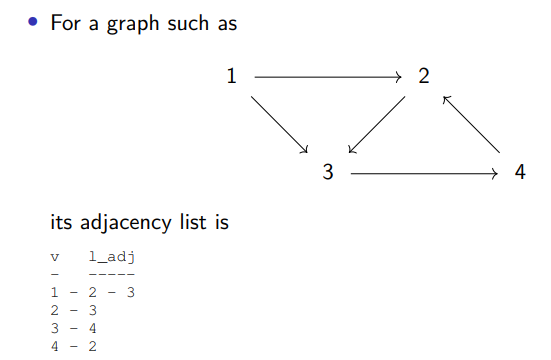
\includegraphics[width = 0.8\textwidth]{figs/graph.png}
\end{figure}

En un grafo, el \textbf{grado de entrada} (in degree) de un vértice es el número de aristas que llegan a él, mientras que el \textbf{grado de salida} (out degree) es el número de aristas que salen de él. En grafos no dirigidos, el grado de un vértice simplemente se refiere al número de aristas incidentes a él.

\subsubsection{El Problema de los Puentes de Königsberg}
El problema de los puentes de Königsberg es un famoso problema matemático que data del siglo XVIII. La ciudad de Königsberg (actualmente Kaliningrado) estaba dividida por el río Pregel, con dos islas conectadas entre sí y con las orillas del río mediante siete puentes. El desafío consistía en encontrar un camino que permitiera cruzar cada puente exactamente una vez y regresar al punto de partida.

Este problema puede modelarse como un \textbf{grafo no dirigido}, donde cada región de la ciudad (orillas e islas) se representa como un vértice, y cada puente como una arista que conecta dos vértices. El objetivo es encontrar un \textbf{camino euleriano}, es decir, un recorrido que pase por cada arista exactamente una vez.

\subsubsection{Condiciones para la Existencia de Caminos Eulerianos}
Un \textbf{camino euleriano} es un recorrido que atraviesa cada arista de un grafo exactamente una vez. Si el camino comienza y termina en el mismo vértice, se denomina \textbf{circuito euleriano}.

Para que un grafo no dirigido tenga un camino euleriano, se deben cumplir las siguientes condiciones:
\begin{itemize}
\item El grafo debe estar conectado (es decir, debe existir un camino entre cualquier par de vértices).
\item Exactamente dos vértices deben tener un grado impar. Estos vértices serán el punto de inicio y el punto final del camino.
\item Todos los demás vértices deben tener un grado par.
\end{itemize}

En el caso de un circuito euleriano, todas las condiciones anteriores se mantienen, excepto que todos los vértices deben tener un grado par, ya que el camino debe comenzar y terminar en el mismo vértice.

\subsubsection{Aplicación al Problema de Königsberg}
En el grafo que representa los puentes de Königsberg, todos los vértices tienen un grado impar. Por lo tanto, no es posible encontrar ni un camino euleriano ni un circuito euleriano. Esto llevó a Leonhard Euler a concluir que no existe una solución al problema original.

Euler no solo demostró que estas condiciones son necesarias, sino también suficientes. Es decir, si un grafo no dirigido cumple las condiciones mencionadas, entonces existe un camino o circuito euleriano.

\subsubsection{Observaciones Adicionales}
En un circuito euleriano, el punto de partida es irrelevante, ya que el recorrido terminará en el mismo vértice. Sin embargo, no todos los puntos de partida permiten recorrer todas las aristas en un camino euleriano que no sea un circuito.

En grafos dirigidos, las condiciones para la existencia de caminos eulerianos son análogas, pero deben considerarse los grados de entrada y salida de cada vértice.

\subsubsection{Caminos hamiltonianos}
Si G es un grafo no dirigido, un camino hamiltoniano es un camino en G que visita cada nodo sólo una vez. Mientras que los caminos eulerianos tenían un coste de $O(|E|)$, encontrar un camino hamiltoniano es mucho más costoso computacionalmente. 

\subsection{Secuenciación del ADN hamiltoniana y euleriana}
El objetivo de la secuenciación del genoma es descomponer un gen en una secuencia de cuatro letras (A, T, G, C). 
A grandes rasgos, la secuenciación Shotgun sigue un proceso de cuatro pasos:
\begin{enumerate}
\item Dividir el gen en lecturas cortas aleatorias de 100-500 bases.
\item Identificar las secuencias de lectura hibridándolas en una micromatriz de ADN.
\item Reconstruir cada lectura a partir de estas secuencias.
\item Reconstruir el gen completo a partir de las lecturas.
\end{enumerate}
Los primeros dos pasos son bioquímica pura, pero el tercer paso se basa en caminos hamiltonianos o eulerianos. 

La hibridación de microarrays funciona de la siguiente forma:
\begin{itemize}
\item Colocar todas las sondas de longitud $l$ posibles, es decir, secuencias de ADN de una longitud $l$ fija, en los puntos de una micromatriz.
\item Colocar una gota de ADN marcado con fluorescencia en cada micropunto de la matriz.
\item El fragmento de ADN se hibrida con las micropuntos que son complementarias a una determinada subsecuencia de longitud $l$ del fragmento. De esta forma obtenemos todas las posibles subsecuencias de longitud $l$ que forman el fragmento pero están desordenadas. Siguen el orden en el microarray pero no el de la secuencia.
\end{itemize}

Llamamos $l$-mero a la secuencia de cada una de las sondas. El $l$-espectro sp(S, $l$) de una secuencia S es el conjunto de todos los $l$-meros de S. Por ejemplo, para S = [TATGGTGC] tenemos sp(S, 3)= {TAT, ATG, TGG, GGT, GTG, TGC}. Después de la hibridación, las sondas hibridadas en el microarray nos dan una versión desordenada de sp(S, $l$) que tenemos que reordenar para recuperar S. Definimos el solapamiento $\omega(s1,s2)$ entre dos $l$-mers s1, s2 como la longitud más larga de un sufijo de s1 que también es un prefijo de s2. Claramente tenemos $\omega(s1,s2) \leq l - 1$. Ahora, si s2 sigue a s1 en S, debemos tener $\omega(s1,s2) = l - 1$.

Se puede reconstruir la secuencia S encontrando y ordenando $s_{i1} \ldots s{ik}$ de $sp(S, l)$ de forma que $\omega(s_{ij}, s{ij+1}) = l - 1$. Esto sugiere definir un grafo $G_l(S) = (V_l, E_l)$ donde $V_l = sp(S, l)$ y $(s, s') \in E_l$ si $\omega(s, s') = l - 1$.
Reconstruir S es equivalente a pasar una vez por todos los nodos de $G_l(S)$. De esta formal, podemos reconstruir S encontrando un camino hamiltoniano en $G_l(S)$.
\begin{figure}[h]
\centering
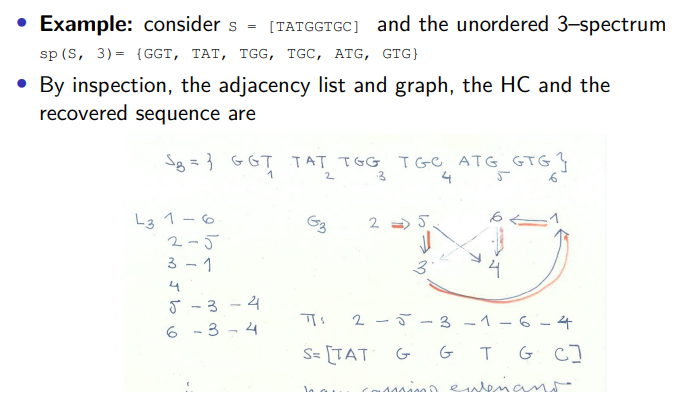
\includegraphics[width = \textwidth]{figs/hamiltonian-dna.png}
\end{figure}

El problema de los caminos hamiltonianos es que son algoritmos muy poco eficientes. La alternativa es intentar hacer $l$-meros en los vértices en lugar de en los nodos. Si $s \in sp(S, l)$ y $\delta_1$ es el prefijo de $l - 1$ y $\delta_2$ su sufijo, podemos considerar s como el vértice que conecta los nodos $\delta_1$ y $\delta_2$. De esta forma tenemos $\omega(\delta_1, \delta_2) = l - 2$. Ahora, podemos definir el grafo $G_{l-1} = (V_{l-1}, E_{l-1})$ donde $V_{l-1} = sp(S, l-1)$ y $(\delta, \delta') \in E_{l-1}$ si son respectivamente prefijo y sufijo de $s \in sp(S, l)$. De esta forma, reconstruir S es equivalente a pasar una vez por todos los vértices de $G_{l-1}$: encontrar el camino euleriano.

Este grafo es dirigido, por lo que hay que adaptar la teoría del camino euleriano a este tipo de grafos. En un grafo dirigido $G(V, E)$ tenemos que distinguir entre vértices incidentes y adyacentes. Por cada $u \in V$, decimos que $(u, v)$ es un vértice adyacente para u e incidente para v. 

\begin{figure}[h]
\centering
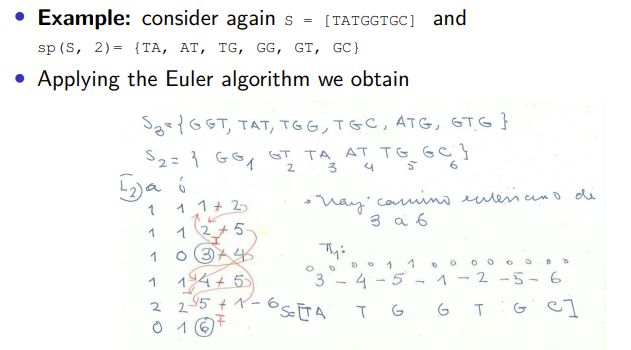
\includegraphics[width = \textwidth]{figs/eulerian-dna.png}
\end{figure}
